\section{Introduction}

% Time series data is ubiquitous in real-world systems and constitutes a fundamental basic for decision-making in numerous application domains. 
% Tasks such as stock price forecasting in finance, patient health monitoring in healthcare, machine condition monitoring in manufacturing, and traffic flow optimization in transportation all rely on accurate time series prediction to uncover underlying temporal patterns and support data-driven decision processes. 
% With the rapid development of deep learning, models such as Recurrent Neural Networks (RNNs), Convolutional Neural Networks (CNNs), and Transformers-based architectures have achieved substantial progress by effectively capturing temporal dependencies and improving forecasting accuracy. 

% Recently, diffusion models have emerged as a powerful class of generative framework and have attracted increasing attention in time series forecasting due to their capacity to model complex data distributions. 
% Several diffusion-based methods have been proposed to progressively refine noisy sequences into structured temporal signals, thereby enhance time series prediction. 
% However, real-world time series often exhibit rich multi-scale characteristics, including long-term trends, periodic patterns, and short-term fluctuations. 
% Standard diffusion models struggle to capture these heterogeneous temporal structures simultaneously. 
% To mitigate this limitation, some studies have incorporated trend-decomposition techniques into diffusion models, demonstrating improved performance gains by explicitly modeling temporal components such as trend, seasonality, and residuals variations.  

% Although recent trend-aware diffusion models have made progress in addressing the multi-scale modeling challenge in time series forecasting, they typically assume fixed-length input windows. This constraint significantly limits their practical applicability in real-world settings, where observed sequences often exhibit variable lengths due to irregular sampling, missing data, or dynamic event horizons.
% To mitigate this limitation, Naiman et al.~\cite{naiman_utilizing_nodate} recently proposed a unified diffusion framework that maps one-dimensional time series into two-dimensional image-like representations, thereby enabling handling of variable-length inputs through standard vision-oriented architectures. While this strategy enhances input flexibility, it treats temporal data as generic spatial grids and fails to adequately preserve the intrinsic sequential ordering, causal dependencies, and temporal continuity that are fundamental to time series. Consequently, critical temporal dynamics—especially long-range correlations and scale-specific patterns—may be distorted or lost during the transformation, undermining the model’s predictive fidelity. 
Time series data is fundamental to decision-making in domains such as finance, healthcare, and transportation. While deep learning models like RNNs, CNNs, and Transformers have advanced time series forecasting, recent work has explored diffusion models for their ability to capture complex temporal distributions. However, real-world series often exhibit multi-scale patterns (trends, seasonality, noise) and variable lengths, posing challenges for standard diffusion approaches. Although trend-decomposition methods improve multi-scale modeling, they typically assume fixed input lengths. To address variable-length inputs, Naiman et al.~\cite{DBLP:conf/nips/NaimanBPAFA24} propose mapping time series to 2D image-like representations. While this enhances input flexibility, it risks distorting temporal continuity and long-range dependencies by treating sequential data as spatial grids.

\begin{figure}
	\raggedleft           
	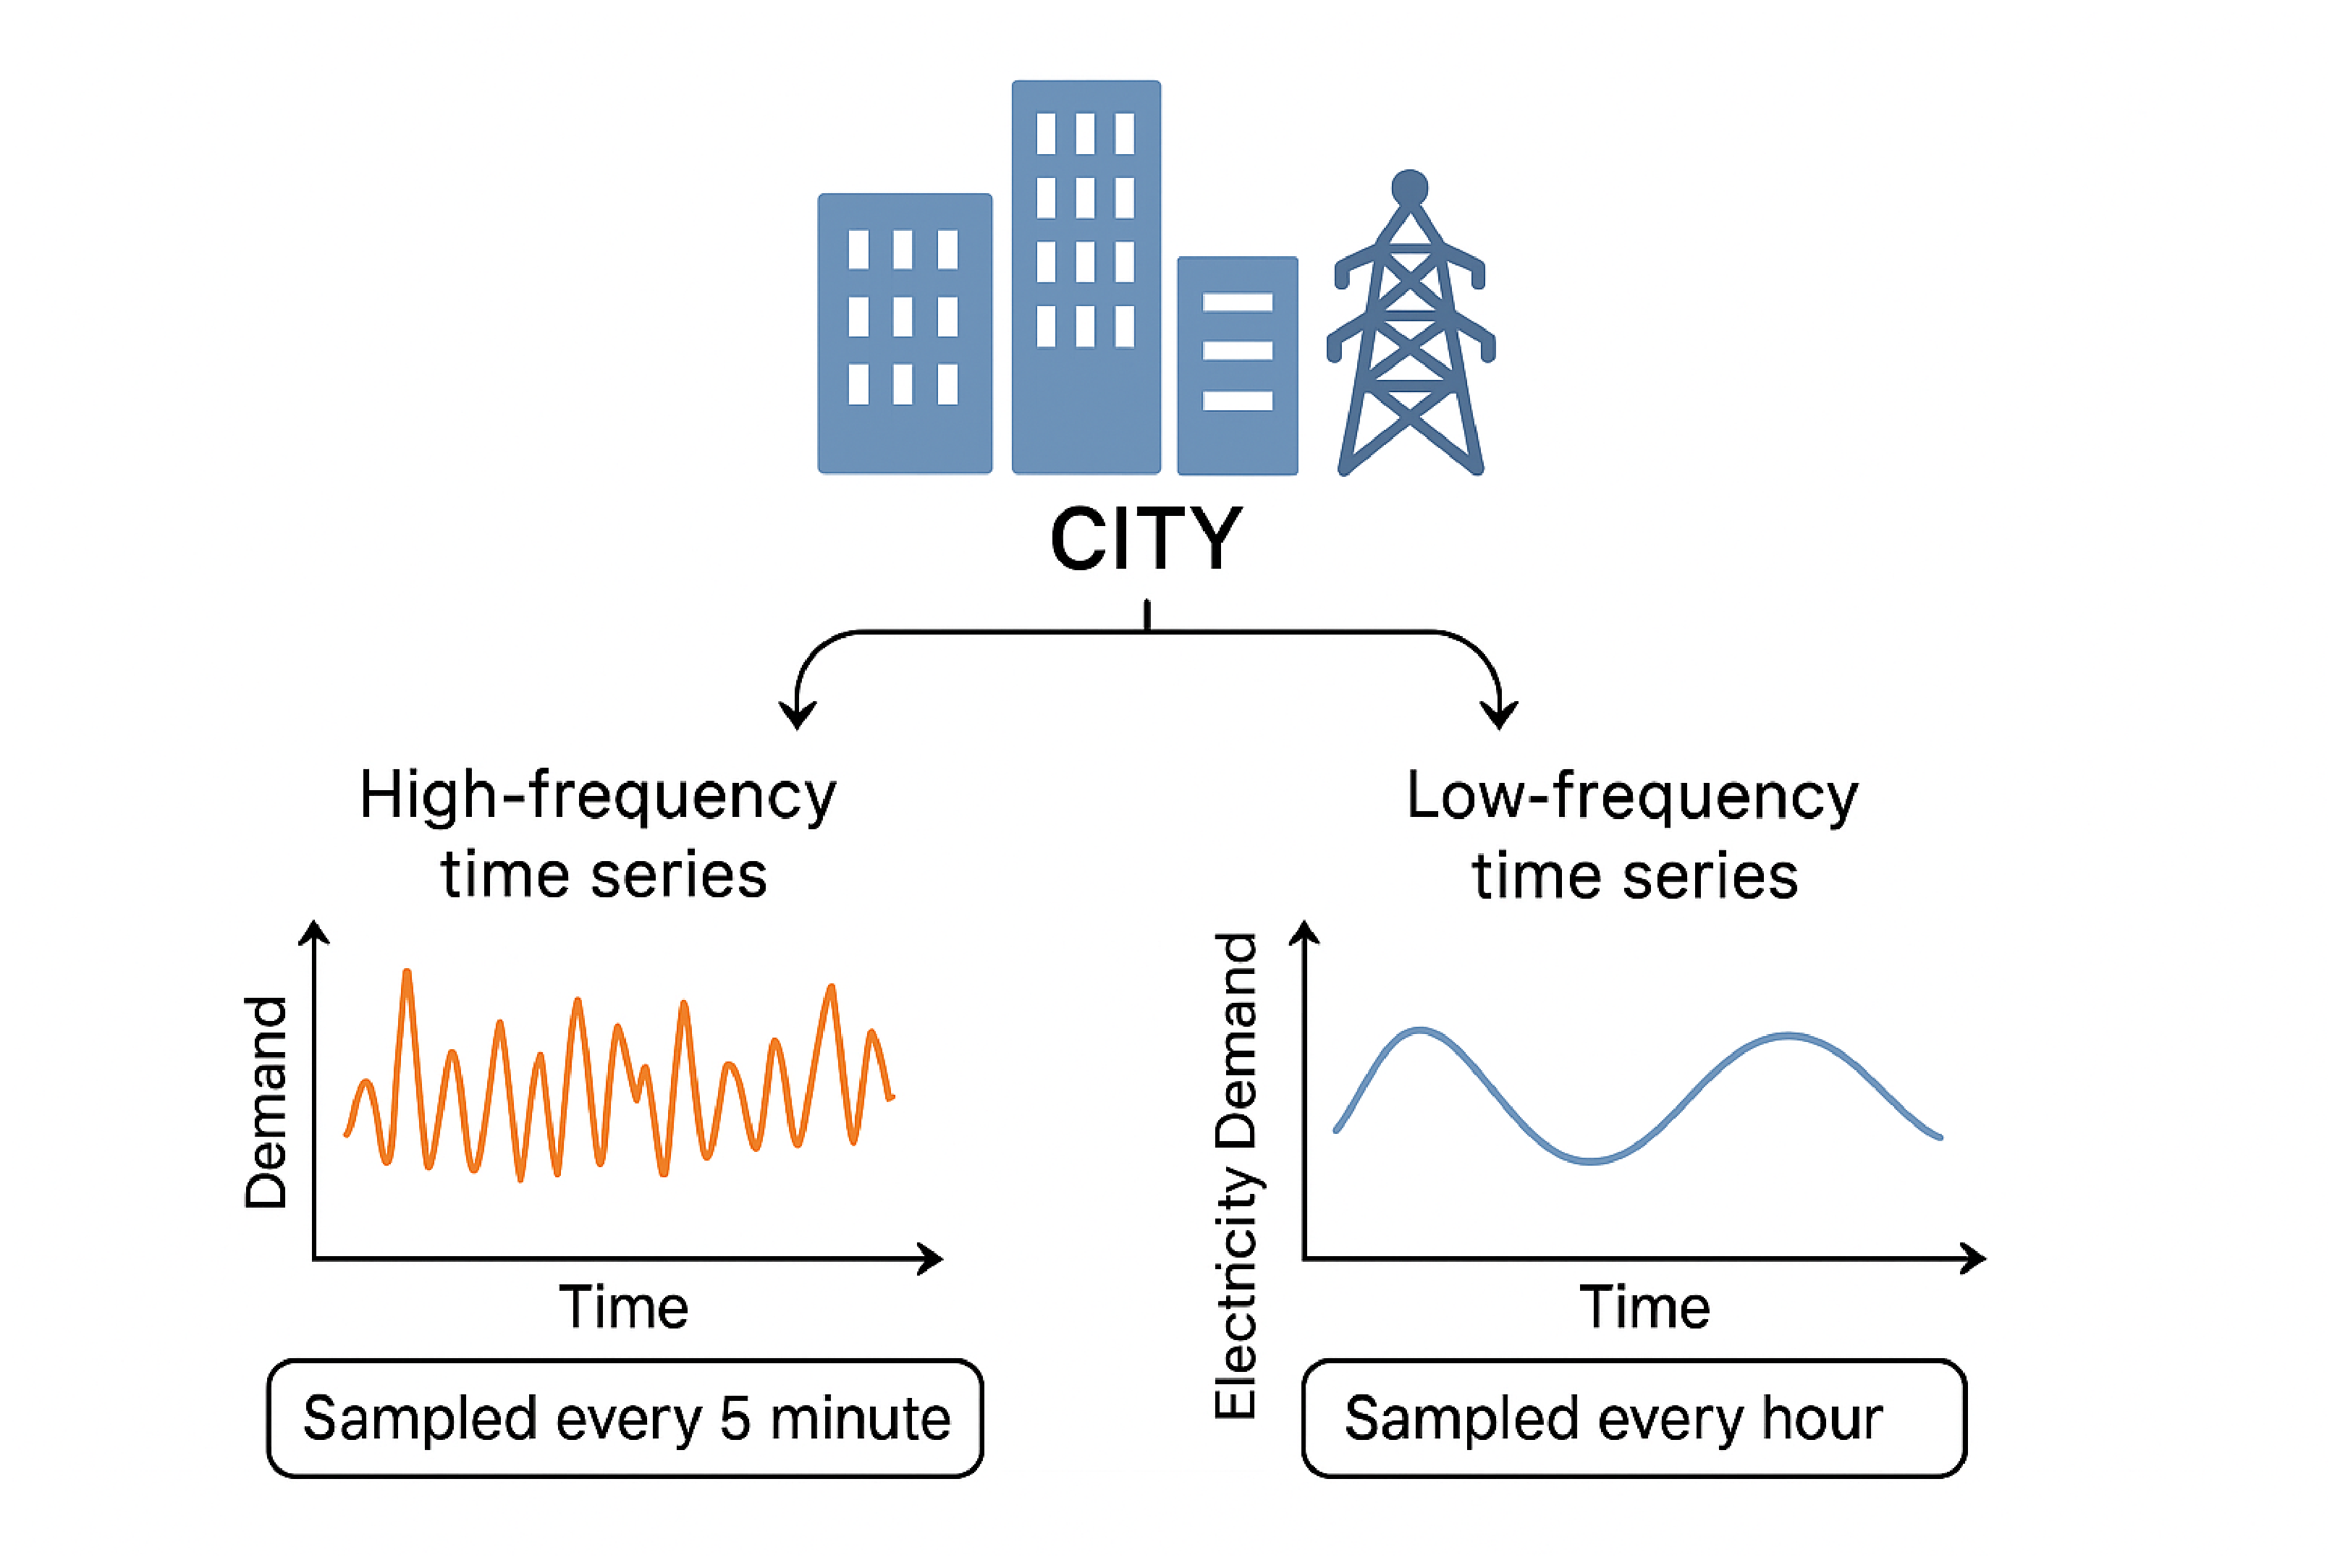
\includegraphics[width=\linewidth]{figures/Ex.eps}
	\caption{Multi-Resolution Time Series Example}
	\label{fig:ex}
\end{figure}
\begin{example}
	% Consider the task of forecasting city-wide electricity demand, where sensors operate at heterogeneous sampling rates--some report measurements every five minutes, while others update only once per hour. 
	% These signals naturally exhibit multi-resolution temporal structures: high-frequency sensors capture rapid, local fluctuations such as household consumption, whereas low-frequency sensors primarily reflect long-term regional trends, including industrial load variations, as illustrated in \autoref{fig:ex}. However, most existing time-series forecasting models--including RNN-, Transformer-, and Diffusion-based architectures--implicitly assume a fixed sampling rate and a single-scale temporal representation. 
	% When heterogeneous signals are forcibly unified into a common temporal resolution through resampling or truncation, models inevitably lose  fine-grained local information or distort global temporal structures, thereby limiting their ability to effectively handle variable-length and inherently multi-scale temporal dynamics.
    Consider forecasting city-wide electricity demand with heterogeneous sampling rates (e.g., 5-minute vs. hourly sensors), as illustrated in \autoref{fig:ex}. High-frequency data captures local fluctuations, while low-frequency data reflects regional trends. However, most models assume fixed sampling rates. Forcing heterogeneous signals into a common resolution inevitably sacrifices fine-grained details or distorts global structures, limiting the ability to handle multi-scale dynamics.
\end{example}
% To address the aforementioned limitations, we propose a novel diffusion-based forecasting framework that simultaneously 
% (1) accommodates variable-length time series without relying on fixed-size input window, and 
% (2) integrates multi-scale trend decomposition to explicitly model temporal structures at different resolutions. 
% Our method preserves the generative advantages of diffusion models while enhancing robustness across heterogeneous sequence length and temporal scales. 
% Comprehensive experiments on multiple real-world datasets demonstrate that our approach consistently outperforms both diffusion-based and conventional forecasting baselines, yielding more accurate and reliable forecasts.
To address these limitations, we propose a diffusion-based forecasting framework that (1) supports variable-length time series without fixed input windows, and (2) incorporates multi-scale trend decomposition to model temporal patterns at different resolutions. The method retains the generative strengths of diffusion models while improving robustness across heterogeneous sequence lengths and temporal scales. Experiments on multiple real-world datasets show that it consistently outperforms both diffusion-based and conventional baselines, achieving more accurate and reliable forecasts.

% 无精简The contributions of this work are summarized as follows:  
% \begin{itemize}[leftmargin=*]
% 	\item We propose a flexible diffusion architecture capable of processing time series of arbitrary lengths, thereby eliminating the fixed-window constraint imposed by most existing forecasting models. 
% 	\item We integrate a hierarchical multi-scale trend decomposition module into diffusion process, enabling explicit modeling of both long-term temporal trends and fine-grained local fluctuations.
% 	\item We conduct comprehensive experiments on multiple real-world datasets, demonstrating the superiority of our method over state-of-the-art time series forecasting models.
% \end{itemize}

The remainder of this paper is organized as follows: 
Section~\ref{sec:related} reviews related literature on time series forecasting and diffusion-based generative models. 
Section~\ref{sec:ps} introduces the problem statement.
Section~\ref{sec:solution} presents the proposed \solutionSimpleName{} framework in detail. 
Section~\ref{sec:experiments} outlines the experimental setup and reports empirical the results. 
Finally, Section~\ref{sec:conclusion} concludes the paper and discusses potential directions for future research.







